\chapter{进程模板}

进程模板定义了协议进程的属性、方法和通信手段,在使用sbid进行协议建模时,进程模板是必不可少的部分。

\section{自定义类型}
在[协议>概览]下,点击小工具栏上的[创建UserType]按钮,即可创建新的自定义类型的类图,如图\ref{usertype}所示。
    \begin{figure}[h]
	\centering
	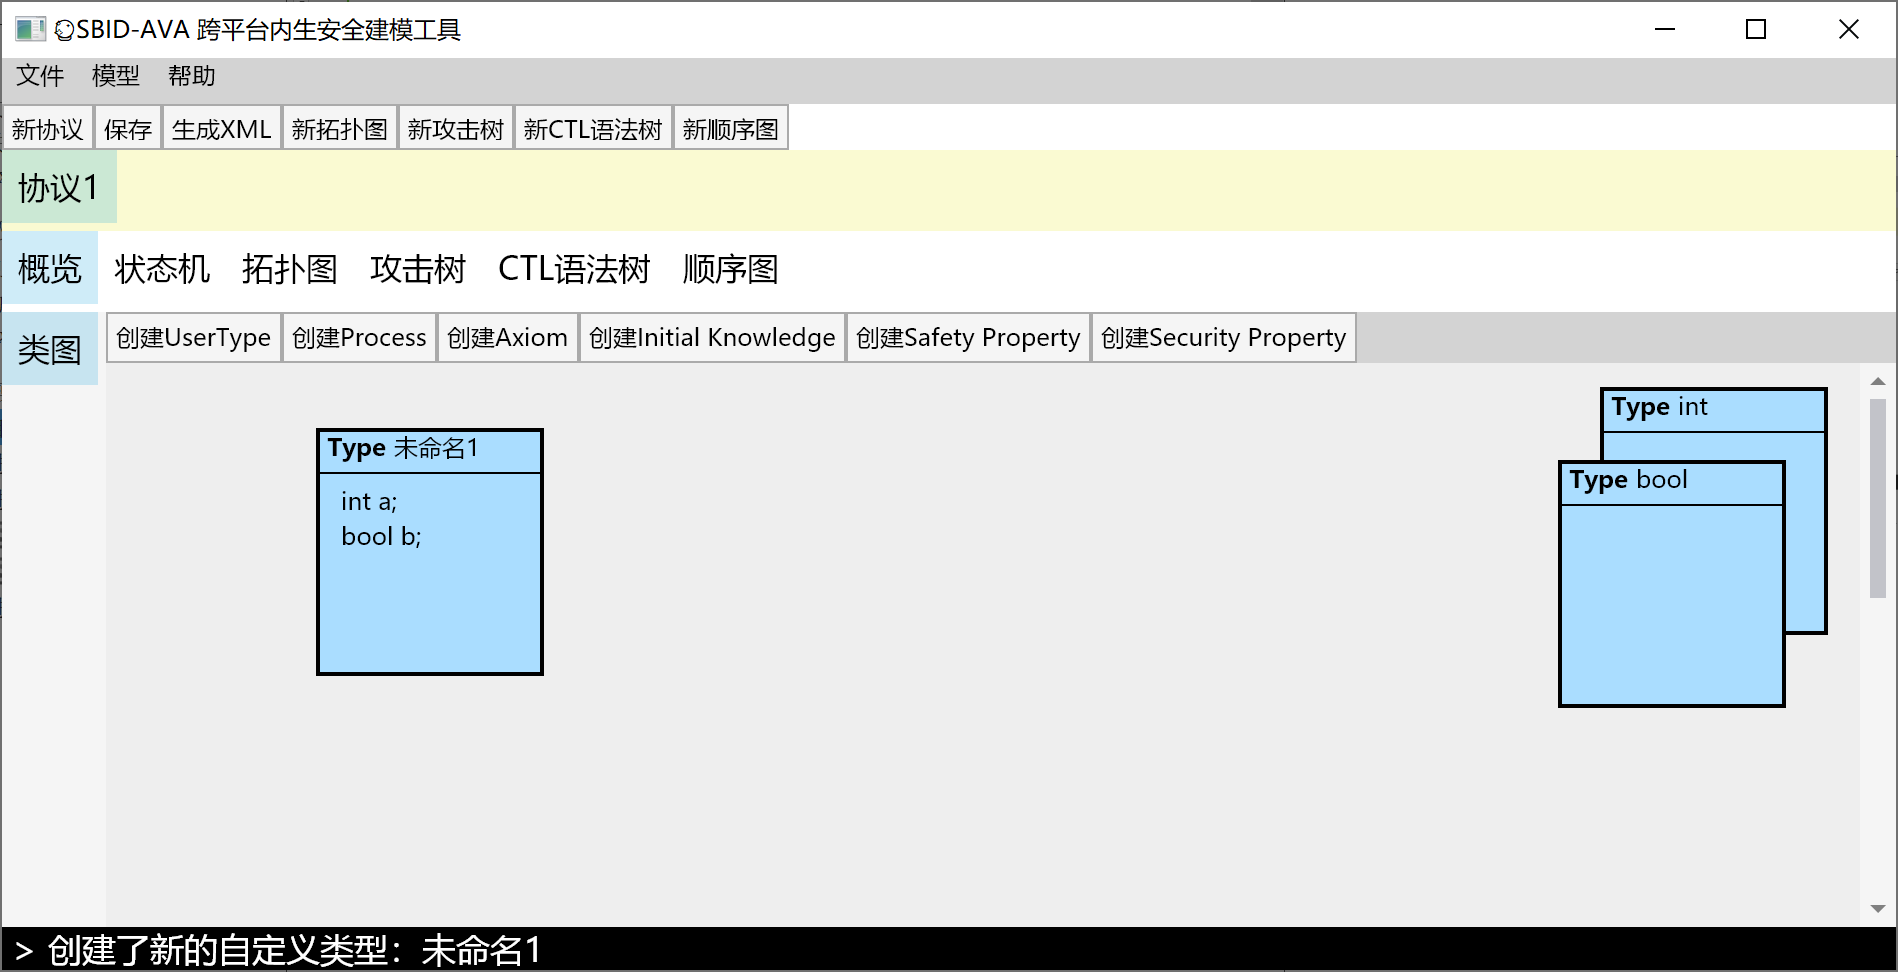
\includegraphics[width=12cm,height=6.75cm]{imgs/usertype.png}
	\caption{新创建的自定义类型}
	\label{usertype}
	\end{figure}
\par
在sbid工具中,默认为用户内置了$int$和$bool$两种基本数据类型,用户可以使用它们定制更为复杂的数据类型,以用于进程模板的构建。
\par
在自定义类型的类图上右键,呼出右键菜单,点击[编辑],即可打开自定义类型的编辑窗体,如图\ref{usertype_edit_window}所示。
\begin{figure}[h]
	\centering
	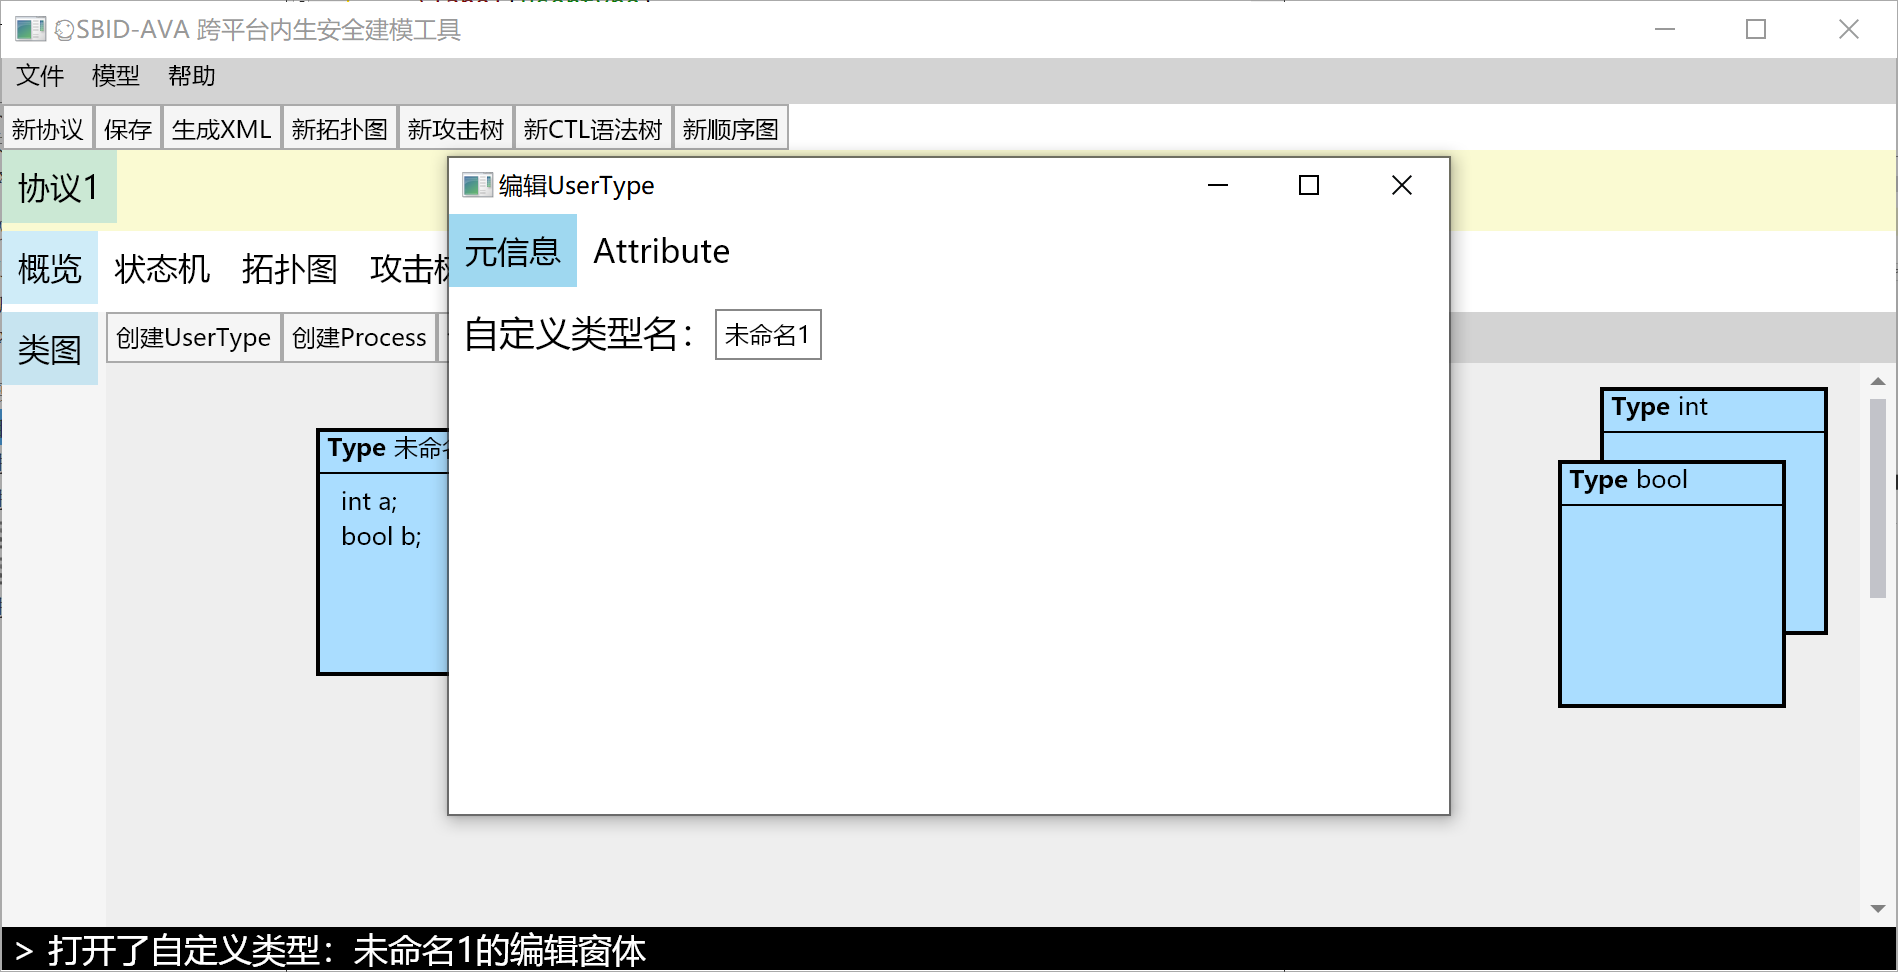
\includegraphics[width=12cm,height=6.75cm]{imgs/usertype_edit_window.png}
	\caption{自定义类型的编辑窗体}
	\label{usertype_edit_window}
\end{figure}
\par
每个自定义类型是以若干个类型为成员的新类型,在左侧选中已有类型,写入字段名称,点击添加按钮即可添加成员变量,如图\ref{usertype_edit_add}所示。
    \begin{figure}[h]
	\centering
	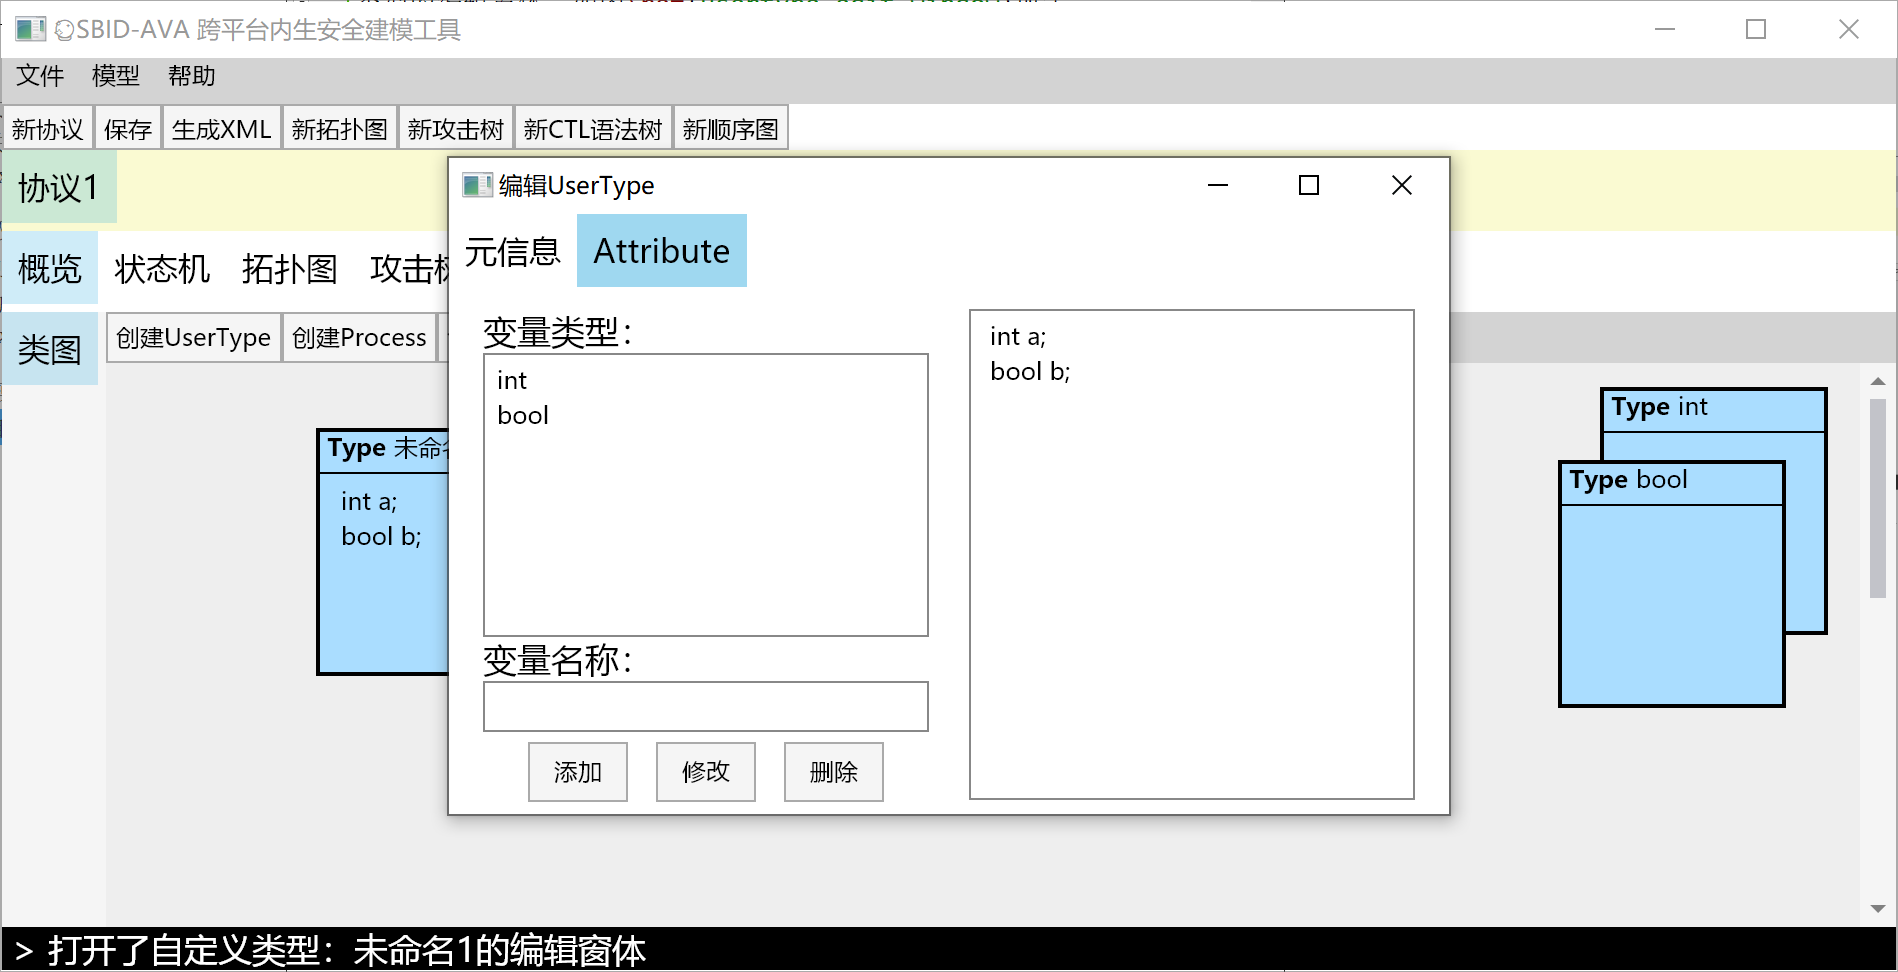
\includegraphics[width=12cm,height=6.75cm]{imgs/usertype_edit_add.png}
	\caption{添加成员变量}
	\label{usertype_edit_add}
	\end{figure}
\par
同理,选中右侧已存在的成员变量,可对其进行修改和删除。
\par
自定义类型可用在进程模板的属性、方法和通信方法的定义上。

